% GNUPLOT: LaTeX picture with Postscript
\documentclass{minimal}
% Set font size
\makeatletter
\def\@ptsize{1}
\InputIfFileExists{size20.clo}{}{%
   \GenericError{(gnuplot) \space\space\space\@spaces}{%
      Gnuplot Error: File `size20.clo' not found! Could not set font size%
   }{See the gnuplot documentation for explanation.%
   }{For using a font size a file `size<fontsize>.clo' has to exist.
        Falling back ^^Jto default fontsize 10pt.}%
  \def\@ptsize{0}
  \input{size10.clo}%
}%
\makeatother
% Load packages
\usepackage{graphicx}
\usepackage{color}
\makeatletter
% Select an appropriate default driver (from TeXLive graphics.cfg)
\begingroup
  \chardef\x=0 %
  % check pdfTeX
  \@ifundefined{pdfoutput}{}{%
    \ifcase\pdfoutput
    \else
      \chardef\x=1 %
    \fi
  }%
  % check VTeX
  \@ifundefined{OpMode}{}{%
    \chardef\x=2 %
  }%
\expandafter\endgroup
\ifcase\x
  % default case
  \PassOptionsToPackage{dvips}{geometry}
\or
  % pdfTeX is running in pdf mode
  \PassOptionsToPackage{pdftex}{geometry}
\else
  % VTeX is running
  \PassOptionsToPackage{vtex}{geometry}
\fi
\makeatother
% Set papersize
\usepackage[papersize={360.00bp,252.00bp},text={360.00bp,252.00bp}]{geometry}
% No page numbers and no paragraph indentation
\pagestyle{empty}
\setlength{\parindent}{0bp}%
% Load configuration file
\InputIfFileExists{gnuplot.cfg}{%
  \typeout{Using configuration file gnuplot.cfg}%
}{%
 \typeout{No configuration file gnuplot.cfg found.}%
}%
%
\begin{document}
\begingroup
  \makeatletter
  \providecommand\color[2][]{%
    \GenericError{(gnuplot) \space\space\space\@spaces}{%
      Package color not loaded in conjunction with
      terminal option `colourtext'%
    }{See the gnuplot documentation for explanation.%
    }{Either use 'blacktext' in gnuplot or load the package
      color.sty in LaTeX.}%
    \renewcommand\color[2][]{}%
  }%
  \providecommand\includegraphics[2][]{%
    \GenericError{(gnuplot) \space\space\space\@spaces}{%
      Package graphicx or graphics not loaded%
    }{See the gnuplot documentation for explanation.%
    }{The gnuplot epslatex terminal needs graphicx.sty or graphics.sty.}%
    \renewcommand\includegraphics[2][]{}%
  }%
  \providecommand\rotatebox[2]{#2}%
  \@ifundefined{ifGPcolor}{%
    \newif\ifGPcolor
    \GPcolortrue
  }{}%
  \@ifundefined{ifGPblacktext}{%
    \newif\ifGPblacktext
    \GPblacktexttrue
  }{}%
  % define a \g@addto@macro without @ in the name:
  \let\gplgaddtomacro\g@addto@macro
  % define empty templates for all commands taking text:
  \gdef\gplbacktext{}%
  \gdef\gplfronttext{}%
  \makeatother
  \ifGPblacktext
    % no textcolor at all
    \def\colorrgb#1{}%
    \def\colorgray#1{}%
  \else
    % gray or color?
    \ifGPcolor
      \def\colorrgb#1{\color[rgb]{#1}}%
      \def\colorgray#1{\color[gray]{#1}}%
      \expandafter\def\csname LTw\endcsname{\color{white}}%
      \expandafter\def\csname LTb\endcsname{\color{black}}%
      \expandafter\def\csname LTa\endcsname{\color{black}}%
      \expandafter\def\csname LT0\endcsname{\color[rgb]{1,0,0}}%
      \expandafter\def\csname LT1\endcsname{\color[rgb]{0,1,0}}%
      \expandafter\def\csname LT2\endcsname{\color[rgb]{0,0,1}}%
      \expandafter\def\csname LT3\endcsname{\color[rgb]{1,0,1}}%
      \expandafter\def\csname LT4\endcsname{\color[rgb]{0,1,1}}%
      \expandafter\def\csname LT5\endcsname{\color[rgb]{1,1,0}}%
      \expandafter\def\csname LT6\endcsname{\color[rgb]{0,0,0}}%
      \expandafter\def\csname LT7\endcsname{\color[rgb]{1,0.3,0}}%
      \expandafter\def\csname LT8\endcsname{\color[rgb]{0.5,0.5,0.5}}%
    \else
      % gray
      \def\colorrgb#1{\color{black}}%
      \def\colorgray#1{\color[gray]{#1}}%
      \expandafter\def\csname LTw\endcsname{\color{white}}%
      \expandafter\def\csname LTb\endcsname{\color{black}}%
      \expandafter\def\csname LTa\endcsname{\color{black}}%
      \expandafter\def\csname LT0\endcsname{\color{black}}%
      \expandafter\def\csname LT1\endcsname{\color{black}}%
      \expandafter\def\csname LT2\endcsname{\color{black}}%
      \expandafter\def\csname LT3\endcsname{\color{black}}%
      \expandafter\def\csname LT4\endcsname{\color{black}}%
      \expandafter\def\csname LT5\endcsname{\color{black}}%
      \expandafter\def\csname LT6\endcsname{\color{black}}%
      \expandafter\def\csname LT7\endcsname{\color{black}}%
      \expandafter\def\csname LT8\endcsname{\color{black}}%
    \fi
  \fi
  \setlength{\unitlength}{0.0500bp}%
  \begin{picture}(7200.00,5040.00)%
    \gplgaddtomacro\gplbacktext{%
      \csname LTb\endcsname%
      \put(900,1170){\makebox(0,0)[r]{\strut{} \small{0}}}%
      \put(900,1684){\makebox(0,0)[r]{\strut{} \small{20}}}%
      \put(900,2199){\makebox(0,0)[r]{\strut{} \small{40}}}%
      \put(900,2713){\makebox(0,0)[r]{\strut{} \small{60}}}%
      \put(900,3227){\makebox(0,0)[r]{\strut{} \small{80}}}%
      \put(900,3741){\makebox(0,0)[r]{\strut{} \small{100}}}%
      \put(900,4256){\makebox(0,0)[r]{\strut{} \small{120}}}%
      \put(900,4770){\makebox(0,0)[r]{\strut{} \small{140}}}%
      \put(1120,900){\makebox(0,0){\strut{} \small{49}}}%
      \put(1499,900){\makebox(0,0){\strut{} \small{50}}}%
      \put(1877,900){\makebox(0,0){\strut{} \small{51}}}%
      \put(2256,900){\makebox(0,0){\strut{} \small{52}}}%
      \put(2635,900){\makebox(0,0){\strut{} \small{53}}}%
      \put(3013,900){\makebox(0,0){\strut{} \small{54}}}%
      \put(3392,900){\makebox(0,0){\strut{} \small{55}}}%
      \put(3771,900){\makebox(0,0){\strut{} \small{56}}}%
      \put(4149,900){\makebox(0,0){\strut{} \small{57}}}%
      \put(4528,900){\makebox(0,0){\strut{} \small{58}}}%
      \put(4907,900){\makebox(0,0){\strut{} \small{59}}}%
      \put(5285,900){\makebox(0,0){\strut{} \small{60}}}%
      \put(5664,900){\makebox(0,0){\strut{} \small{61}}}%
      \put(6043,900){\makebox(0,0){\strut{} \small{62}}}%
      \put(6421,900){\makebox(0,0){\strut{} \small{63}}}%
      \put(6800,900){\makebox(0,0){\strut{} \small{64}}}%
      \put(200,4900){\rotatebox{-270}{\makebox(0,0)[r]{\strut{}\# of events}}}%
      \put(7050,300){\makebox(0,0)[r]{\strut{}Strip}}%
    }%
    \gplgaddtomacro\gplfronttext{%
      \csname LTb\endcsname%
      \put(4774,4602){\makebox(0,0)[r]{\strut{}}}%
      \csname LTb\endcsname%
      \put(4774,4382){\makebox(0,0)[r]{\strut{}}}%
      \csname LTb\endcsname%
      \put(4774,4162){\makebox(0,0)[r]{\strut{}}}%
      \csname LTb\endcsname%
      \put(4774,3942){\makebox(0,0)[r]{\strut{}}}%
    }%
    \gplbacktext
    \put(0,500){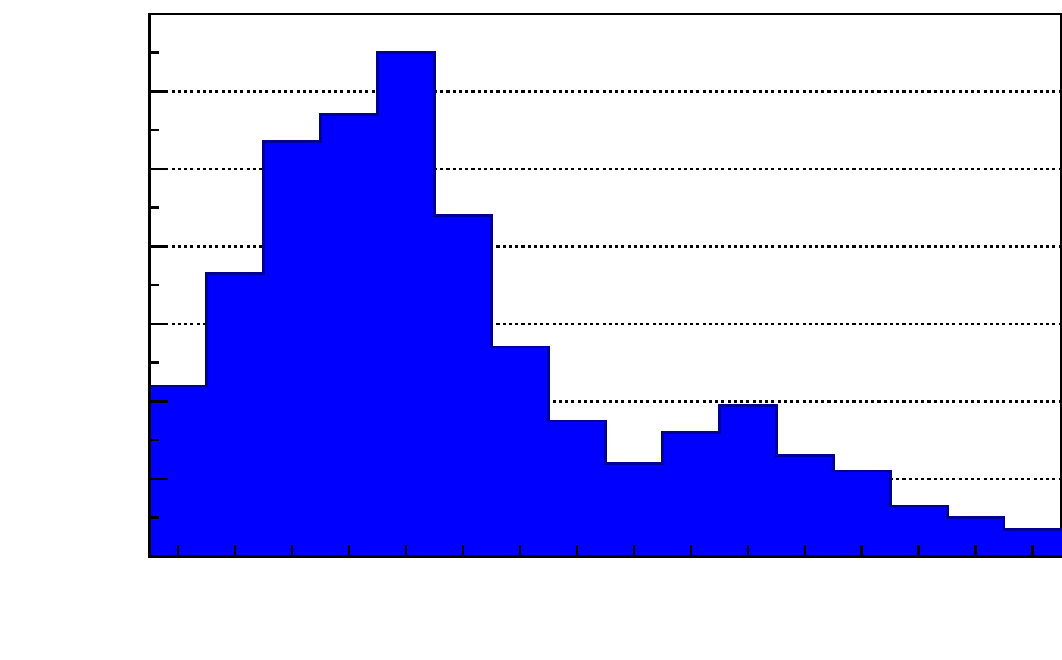
\includegraphics[scale=0.691]{B2-inc}}%
    \gplfronttext
  \end{picture}%
\endgroup
\end{document}